% Template for Cogsci submission with R Markdown

% Stuff changed from original Markdown PLOS Template
\documentclass[10pt, letterpaper]{article}

\usepackage{cogsci}
\usepackage{pslatex}
\usepackage{float}
\usepackage{caption}

% amsmath package, useful for mathematical formulas
\usepackage{amsmath}

% amssymb package, useful for mathematical symbols
\usepackage{amssymb}

% hyperref package, useful for hyperlinks
\usepackage{hyperref}

% graphicx package, useful for including eps and pdf graphics
% include graphics with the command \includegraphics
\usepackage{graphicx}

% Sweave(-like)
\usepackage{fancyvrb}
\DefineVerbatimEnvironment{Sinput}{Verbatim}{fontshape=sl}
\DefineVerbatimEnvironment{Soutput}{Verbatim}{}
\DefineVerbatimEnvironment{Scode}{Verbatim}{fontshape=sl}
\newenvironment{Schunk}{}{}
\DefineVerbatimEnvironment{Code}{Verbatim}{}
\DefineVerbatimEnvironment{CodeInput}{Verbatim}{fontshape=sl}
\DefineVerbatimEnvironment{CodeOutput}{Verbatim}{}
\newenvironment{CodeChunk}{}{}

% cite package, to clean up citations in the main text. Do not remove.
\usepackage{apacite}

% KM added 1/4/18 to allow control of blind submission
\cogscifinalcopy

\usepackage{color}

% Use doublespacing - comment out for single spacing
%\usepackage{setspace}
%\doublespacing


% % Text layout
% \topmargin 0.0cm
% \oddsidemargin 0.5cm
% \evensidemargin 0.5cm
% \textwidth 16cm
% \textheight 21cm

\title{Active? Associative?: Preschool children assess the feasibility
of a goal based on the acoustic environment}



\newlength{\cslhangindent}
\setlength{\cslhangindent}{1.5em}
\newenvironment{CSLReferences}%
  {}%
  {\par}

\begin{document}

\maketitle

\begin{abstract}
Despite the unpredictible and ubiquitous nature of noise in the natural
environment, most children still manage to extract the linguistic,
cognitive, and social skills needed to engage typically with the world
around them. This is no small feat; it is still largely unknown what
strategies children use to extract information from their environment in
the presence of noise. One possbility is that children have learned how
to reason about their acoustic context to optimize goals and goal
outcomes. In Experiment 1, we presented preschool children with a set of
auditory stimuli, meant to approximate various acoustic environments,
and activity goals to complete within those environments. Results showed
that children reliably integrated auditory information with a
third-party's changing goals to optimize another person's outcomes.
Experiment 2 built on this framework by replacing familiar activity
goals with novel ones to assess the flexibility of children's
decision-making, and offers some preliminary findings.

\textbf{Keywords:}
active learning; associative learning; auditory noise; cognitive
development; decision making
\end{abstract}

\hypertarget{introduction}{%
\section{Introduction}\label{introduction}}

Children are excavators; they routinely build linguistic, cognitive,
social, and emotional skills through interacting with their
environments. They can adjust their attention to linguistic stimuli such
as grammar based on its present learnability (Gerken, Balcomb, \&
Minton, 2011). They can exploit the emotional expressions of others to
determine whether a novel object is worth exploration, thereby
maximizing efficiency (Wu \& Gweon, 2021). And when they do explore,
children are often accounting for both the structure of the environment
and their present goals to decide on a reasonable approach (Meder, Wu,
Schulz, \& Ruggeri, 2021). This flexibility in the learning system is
highly adaptive, as it offers a means for data extraction even in
unfamiliar or suboptimal learning conditions.

We can understand why children are such flexible learners across a
diverse range of environments through the lens of active learning. In
this account, children make decisions about what and how they learn,
which contrasts with the more passive view that they merely absorb
information presented to them without an opportunity to make adjustments
(Raz \& Saxe, 2020). The active learning literature has typically
explored children's interactions with individual stimuli within the
environment (e.g., Settles, 2009). For example, previous work has shown
that preschool children use active learning strategies to approach
objects in a novel task in order to optimize performance (Ruggeri,
Swaboda, Sim, \& Gopnik, 2019). In this task, children either opened or
shook two sets of boxes, one of which contained an egg shaker. When
children were told that the egg shaker was equally likely to be found in
either set of boxes, they were more likely to shake the boxes first than
when they were told the shaker was more likely to be found in a
particular set of boxes. Even infants harness the utility of active
learning by updating their expectations about what could be learned from
an object that behaved unexpectedly, such as a ball moving through a
solid wall (Stahl \& Feigenson, 2015). Additionally, infants as young as
7 months have been shown to efficiently allocate their attention to
visual stimuli that are neither too complex nor too simple (Kidd,
Piantadosi, \& Aslin, 2012).

A traditional account of active learning considers how children engage
with individual stimuli within their environment to harness new
information. But more recent work has considered how children reason
about the environmental structure for learning as well. This type of
active learning has been defined as ecological active learning, and it
requires children to both identify features of their environment that
are stable but influential, and then adjust their exploration strategies
to maximize learning within this ecology (Ruggeri, 2022). Ecological
active learning proposes that the very structure of the environment, and
not merely individual stimuli within it, is critical for
information-seeking. Without a consideration for the constraints of the
environment itself, it may be difficult to maximize efficiency and
obtain new information.

Ecological active learning encourages an emphasis on environmental
features that impact exploration. Given that children with access to
auditory input can learn a great deal from their acoustic environment,
is it also possible that they can reason about how well their acoustic
environment supports goal optimization? In other words, what if children
are using acoustic information from the environment to decide how to
interact with the environment?

An acoustic environment can be flexibly defined, so we refer to it as
the physical space in which the child interacts both in and on, and one
that moves with the child. In this environment, children may adjust
their engagement based on both auditory information and previously
defined goals. For example, a child might choose to read or be read to
in a library or in an empty room because a quiet space best aligns with
the goal of taking in a storybook. We refer to this as environmental
selection, the preferential process of selecting environments that align
with goal optimization. It is preferential because it necessitates that
children prioritize learning opportunities that are best suited for the
present environment. This means that children identify a range of
possible learning opportunities within the current environmental
structure. They then constrain this range to those that can be optimized
by maximizing learnability or efficiency, or by reducing uncertainty.
Environmental selection is also goal-directed; children integrate
information about their environment because they are motivated to
achieve some outcome. Importantly, direct control over the environment
is not a requisite for environmental selection. Instead, it suggests
that given the present environment and having no intervening power on
it, children will engage in activities that align with this environment,
and they will exploit the variation across environments to achieve a
range of goals that would have been less efficient under a single set of
conditions.

Environmental selection emphasizes acoustic information because it is
both a salient feature of an environment and can have cascading effects
on learning and development. The latter is especially true given the
potential for auditory noise which may disrupt learning. We define noise
here as any stimulus that is unwanted or unattended to by the listener,
and can be either internal to the system {[}i.e.~errors in production or
perception, or a limited linguistic repertoire{]}, or external
{[}i.e.~the chatter of a busy coffee shop on Friday afternoon{]}
(Gibson, Bergen, \& Piantadosi, 2013; Shannon, 1948). Noise in the
auditory channel has serious implications for active learning,
especially for young children. Children are notably worse than adults at
skills such as speech perception and word recognition in noise
(Bjorklund \& Harnishfeger, 1990; Klatte, Bergström, \& Lachmann, 2013),
and exhibit real challenges in word learning under background noise
constraints (McMillan \& Saffran, 2016). Because noise generally
increases cognitive load during certain attention and spatial tasks,
children are less able to flexibly adapt strategies to successfully
complete these tasks than adults (Loh, Fintor, Nolden, \& Fels, 2022).
There is also emerging evidence that high levels of sustained noise
exposure changes the cortical thickness of the left inferior frontal
gyrus in infants (Simon, Merz, He, \& Noble, 2022). Importantly, these
effects of noise are not happening exclusively at the unconscious level;
even young children are perceptually aware of excessive noise exposure
(McAllister, Rantala, \& Jónsdóttir, 2019). With this in mind, we
propose that environmental selection may be an adaptive strategy for
learning in a variety of acoustic environments.

In the current paper, we studied both whether and how preschool children
use environmental selection for goal optimization. In Experiment 1, we
asked children to match a set of goals to one or more auditory
environments where appropriate. Then in Experiment 2, we presented
children with novel activities and asked them to complete the same task
to explore the conceptual boundaries of this ability. Taken together,
this set of experiments aims to expand our understanding of how children
can exploit their acoustic environment for goal optimization across a
range of inputs.

\hypertarget{experiment-1}{%
\section{Experiment 1}\label{experiment-1}}

In our first experiment, we evaluated preschool children's environmental
selection, their integration of both auditory information and a third
party's goals, for familiar activities. We asked whether they would
differentially select environment-goal pairings that optimized another
person's goals. If children are systematically pairing based on
outcomes, this may suggest that they are, in fact, attuned to the
environment as a strategy for goal optimization.

\hypertarget{methods}{%
\subsection{Methods}\label{methods}}

\hypertarget{participants}{%
\subsubsection{Participants}\label{participants}}

73 children (3;0 - 5;11 years, mean age = 4.45 years , 27.4\%
Caucasian/White) were recruited from either a local Bay Area nursery
school or children's museum. Participants were typically developing, had
normal or corrected-to-normal vision, and heard English at least 75\% of
the time at home. An additional 4 children were ultimately excluded from
analysis due to response bias (provided the same pattern of responses
for 100\% of trials), experimenter error, or severe lapses in attention.
Caregivers provided written consent while children provided verbal
assent before participation.

\hypertarget{materials-and-procedure}{%
\subsubsection{Materials and Procedure}\label{materials-and-procedure}}

\begin{CodeChunk}
\begin{figure}[t]

{\centering 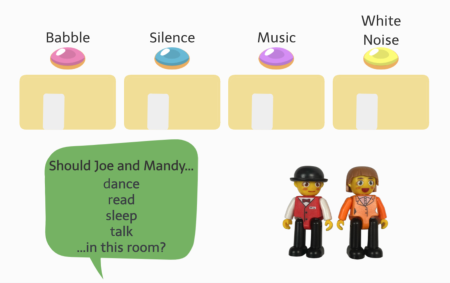
\includegraphics{figs/e3-stimuli-1} 

}

\caption[Experimental setup and stimuli]{Experimental setup and stimuli. Participants were shown four wooden houses, each with an associated sound [instrumental music, multi-talker babble, silence, and white noise], and a list of four activities [dance, read, sleep, talk] that two charactrs in the game wanted to complete. Participants determined whether the two characters should or should not complete an activity in each of the four houses. Responses were independent of each other.}\label{fig:e3-stimuli}
\end{figure}
\end{CodeChunk}

A trained undergraduate research assistant served as the experimenter
for the task. The experimenter first introduced participants to two
small plastic figures named Joe and Mandy and to four wooden houses with
a felt door on the front. The experimenter then showed participants a
list of four images, each depicting one activity Joe and Mandy wanted to
do together. The experimenter explained that when the door opened, each
house would either play a sound or it wouldn't play anything at all. Joe
and Mandy could choose whether or not to complete an activity in each
house, and their decisions would be entirely based on participants'
responses. Importantly, these decisions were independent of each other;
participants could decide to have Joe and Mandy complete the same
activity in more than one room if appropriate. A sound button was
attached to the back of each house and hidden from the participant's
view so when the experimenter opened the door, they also pressed down on
the button to play the appropriate sound. The wooden houses were lined
up on a table several inches apart with the participant seated facing
the door of the house and the experimenter on the opposite side facing
the sound buttons. Figure 1 illustrates the setup, the four activities,
and the four auditory stimuli.

The experimenter began the task with the first image on the list and
told participants, ``It looks like Joe and Mandy want to {[}sleep{]}.
Let's look at each room and see if Joe and Mandy should {[}sleep{]}
inside.'' The experimenter then opened the door to the first house
{[}the experimenter always began with the first house on their left/the
first house on the participant's right{]} and pressed down on the sound
button. At the end of the audio clip, the experimenter closed the door
and asked participants two questions. Participants only heard each audio
once per trial. The experimenter repeated this process for the three
remaining houses before moving on to the next activity. In total,
participants completed 16 trials- 4 trials for each activity times 4
trials for each auditory stimulus. Trials were counterbalanced such that
the presentation order was randomized into four conditions.

Each auditory stimulus was 7s in length and equalized to a root mean
square (RMS) of 65dB. The multi-talker babble was an overlay of five
adult native English speakers reading short, unrelated sentences
(Panfili (n.d.)). The white noise was engineered in Audacity. The
instrumental music contained no human speech. Both the activities and
auditory stimuli were selected based on a sample of adults run
previously. One possible confound is the auditory stimuli suggests
varying numbers of people inside the wooden houses. For example, the
house paired with multi-talker babble may appear to have more figures or
people inside than the houses paired with instrumental music, silence,
and white noise. This may inadvertently influence children's decisions
on whether or not a house is appropriate for a specific activity for
reasons other than the auditory stimuli. To address this, we opened the
top of each house and showed children that two other figures were
inside.

We asked participants two questions which served as our DVs: (1)
``Should Joe and Mandy {[}read/dance/sleep/talk{]} in this room?'' and
(2) ``Why did you say Joe and Mandy {[}should/shouldn't{]}
{[}read/dance/sleep/talk{]} in this room?''

\hypertarget{results-and-discussion}{%
\subsection{Results and Discussion}\label{results-and-discussion}}

\begin{CodeChunk}
\begin{figure*}[t]

{\centering 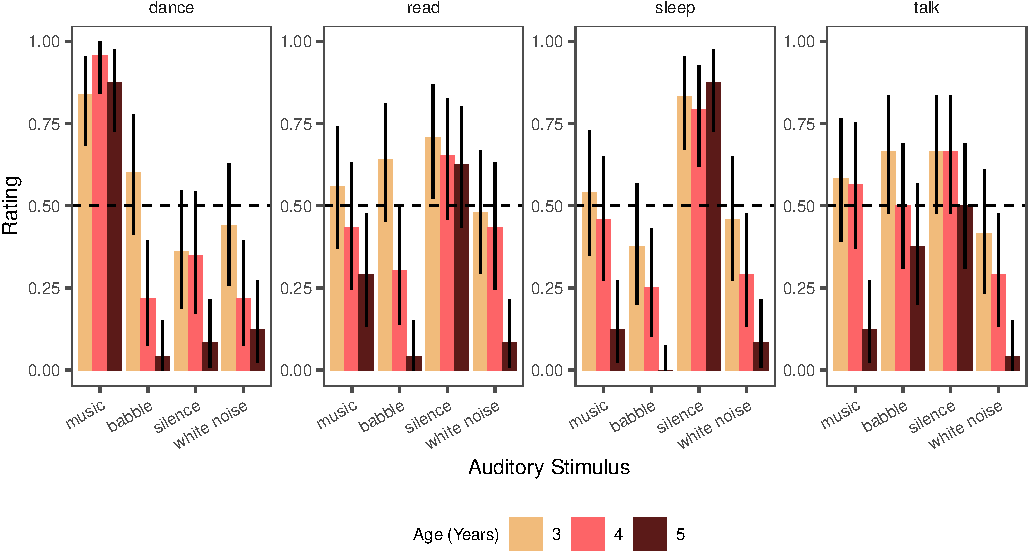
\includegraphics{figs/e3b-bar-1} 

}

\caption[Results from Experiment 1]{Results from Experiment 1. Participants' rating of the appropriateness of an auditory stimulus and activity pairing. Individual bars correspond to one age bin of 3, 4, or 5. A rating score of 0 indicates a rejection of the pairing [Joe and Mandy should not complete a particular activity in this environment] while a score of 1 indicates an affirmation of the pairing [Joe and Mandy should complete a particular activity in this environment]. A 2-alternative forced choice design resulted in no preference at 50\%.  Error bars show 95\% confidence intervals.}\label{fig:e3b-bar}
\end{figure*}
\end{CodeChunk}

If preschool children can reason about how the acoustic environment
might influence goal optimization, and can make decisions to this end,
we should expect participants to show clear preferences for activities
paired with particular auditory stimuli. We preregistered
{[}retracted{]} a Bayesian mixed-effects logistic regression from the
\texttt{rstanarm} package to predict participants' response as a
function of auditory stimulus, activity, and age, with a maximal random
effect structure (random intercept by participant) (Goodrich, Gabry,
Ali, \& Brilleman, 2020). In this and subsequent models, we used the
package default of weakly informative priors (normal distributions on
coefficients with SD=2.5, scaled to predictor magnitudes).

Figure 2 depicts children's activity-auditory pairings by age. We
compared our model {[}activity and auditory stimulus as interactions{]}
with a model with no interaction terms. A one-way ANOVA found that, on
average, the interaction terms better predicted children's responses
during the task {[}\(X^2\)(9) = 165.23, p \textless{} 0.001{]}.

These findings suggest that across the preschool years, children are
evaluating the acoustic environments to make decisions about third-party
goal optimization. We propose that this is evidence of basic
environmental selection, and that children as young as three can
reliably engage in it.

\hypertarget{experiment-2}{%
\section{Experiment 2}\label{experiment-2}}

In Experiment 1, we found that preschool children do engage in
environmental selection, such that they may make decisions about optimal
environments for goal selection based on auditory information. We also
found that this ability was generally stable across the preschool years.
However, it is possible that children succeeded in this task not because
they were engaging in some cognitively flexible process, but because
they were relying on pure associations. For example, children may have
paired napping with silence because they have learned that any sleeping
activity is best done in quiet, and not because they recognize that
silence might be the most optimal auditory environment to both fall and
stay asleep.

Young children harness associative learning in a host of contexts. For
example, associative models of word learning suggest that children
exploit contextual information to acquire the meanings of novel words
(Sloutsky, Yim, Yao, \& Dennis, 2017). This is especially helpful given
referential uncertainty of unfamiliar words that co-occur with other
referents with varying individual probabilities (Quine \& Van, 1960).
Some of the most convincing associative models of word learning are
probabilistic at their core and suggest that word learning happens, in
part, because learners are constantly assessing the probabilities that a
word's meaning is associated with an unfamiliar word. Moreover, these
probabilities are updated as the lexicon expands (see Stevens, Gleitman,
Trueswell, \& Yang, 2017). But associative learning is not relegated to
language development; indeed, humans can develop associative links from
third-party social interactions (Thiele, Hepach, Michel, Gredebäck, \&
Haun, 2021), to remember sequences of stimuli without overloading our
cognitive system (Tosatto, Fagot, Nemeth, \& Rey, 2022), and even to
recognize potential environmental threats, such as snakes and spiders,
in infancy (Rakison, 2022). One possibility, then, is that environmental
selection is driven by associative learning for young children.

While some unifying accounts of active and associative learning exist
(see Kruschke, 2008), traditional associative accounts view the learner
as a passive agent, one who learns what is true about their environment
but does not necessarily act on their environment. It is possible that
reasoning about the acoustic environment, while beneficial, is not
necessary for goal optimization. In other words, perhaps children can
still reach the same decision point with association alone. To test
this, we replaced the familiar activities in Experiment 1 with novel
ones. If children primarily reason about the pairing between the
acoustic environment and a set of goals through pure association, they
should have trouble pairing acoustic environments with novel activities
because they have not previously reasoned about these pairings. If,
however, children are actively updating information about their
environment and then using this information to inform new goals, they
should also succeed even when faced with goals they have never
encountered.

\hypertarget{methods-1}{%
\subsection{Methods}\label{methods-1}}

\hypertarget{participants-1}{%
\subsubsection{Participants}\label{participants-1}}

20 children (3;0 - 5;11 years, mean age = 4.44 years, 40\%
Caucasian/White) were recruited from either a local Bay Area nursery
school or children's museum. An additional 7 children were ultimately
excluded from analysis.

\hypertarget{materials-and-procedure-1}{%
\subsubsection{Materials and
Procedure}\label{materials-and-procedure-1}}

The procedures for Experiment 2 were nearly identical to Experiment 1
with one notable difference. To determine whether preschool children use
environmental selection flexibly to novel activities, we presented
participants with a new list of activities- (1) Fraw: when someone reads
you a bedtime story right before you fall asleep, (2) Gobb: when you are
looking for something to do because you are really bored, (3) Plip: when
you spin around in circles to the beat until you get really dizzy, and
(4) Terb: when you don't want anyone else to know your tummy is making
noise. We selected these novel activities based on an adult sample we
previously ran online, where we found these four activities elicited the
widest distribution of responses among participants.

We asked participants two questions which served as our DVs: (1)
``Should Joe and Mandy {[}fraw/gobb/plip/terb{]} in this room?'' and (2)
``Why did you say Joe and Mandy {[}should/shouldn't{]}
{[}fraw/gobb/plip/terb{]} in this room?''

\hypertarget{results-and-discussion-1}{%
\subsection{Results and Discussion}\label{results-and-discussion-1}}

\begin{CodeChunk}
\begin{figure*}[t]

{\centering 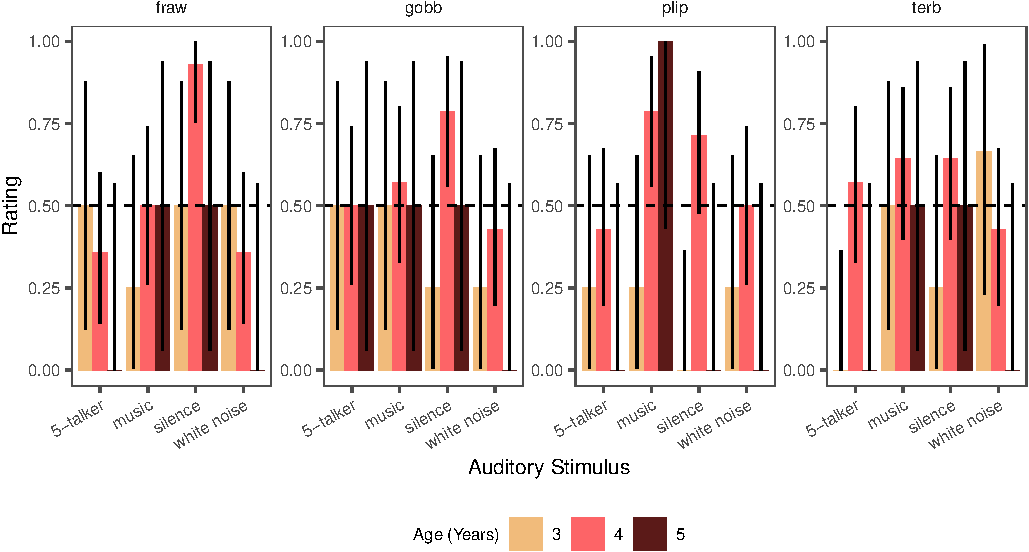
\includegraphics{figs/e4b-bar-1} 

}

\caption[Results from Experiment 2]{Results from Experiment 2. Data is collapsed acrossed age.}\label{fig:e4b-bar}
\end{figure*}
\end{CodeChunk}

\begin{CodeChunk}
\begin{figure*}[t]

{\centering 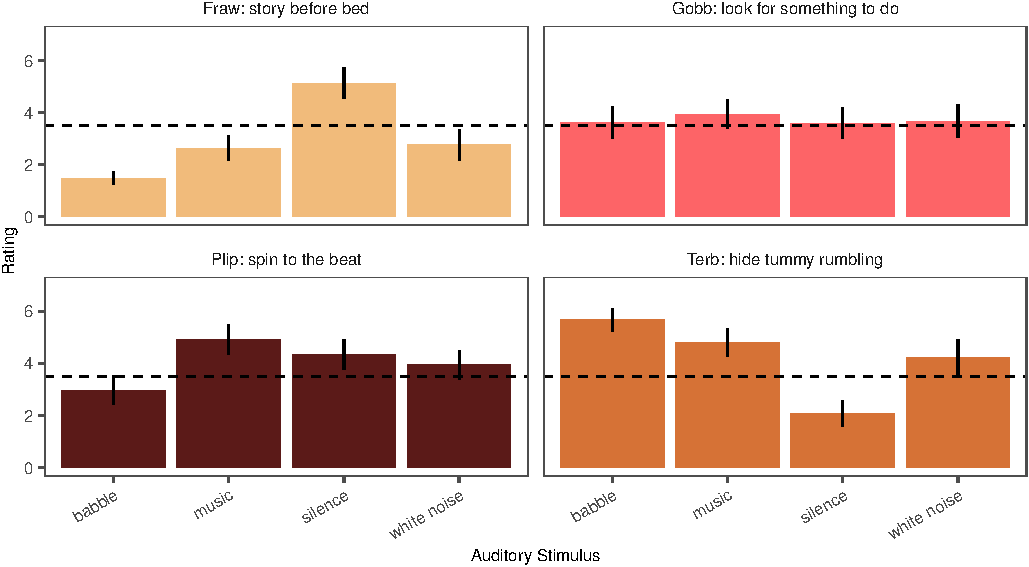
\includegraphics{figs/e4a-bar-1} 

}

\caption[Results from an adult sample]{Results from an adult sample. Adult participants completed the same task as children in Experiment 2, but instead of reasoning about a third party (Joe and Mandy in Exp. 2), they were asked how well they could complete each activity based on the ausitory stimulus. The y-axis indicates the rating scale from 1-7. A rating of 1 denotes a full mismatch between activity and auditory stimulus while 7 denotes an optimal match.}\label{fig:e4a-bar}
\end{figure*}
\end{CodeChunk}

If preschool children rely solely on association when evaluating the
acoustic environment, that is, they have acquired associative links
between familiar activities and their acoustic contexts, we should
expect that children will have no strong preferences for pairing novel
activities with any particular acoustic context. If, however, children
can reason flexibly about how the acoustic environment influences goal
optimization and outcomes, we should expect that children show clear
preferences for acoustic contexts even with activities they have never
actually encountered.

Data collection for Experiment 2 is ongoing, so we present a subset
{[}20 of the preregistered 72-participant sample{]} of the data for
preliminary analysis. Our model with an interaction between activity and
auditory stimulus was not different from a model with no interaction
term {[}\(X^2\)(9) = 12.38, p = 0.19{]}. Figure 3 shows the aggregated
data across all participants.

\hypertarget{adult-ratings-of-novel-activity-pairings}{%
\subsection{Adult Ratings of Novel Activity
Pairings}\label{adult-ratings-of-novel-activity-pairings}}

The previous findings suggest some differentiation in pairing auditory
stimuli with novel activities, but what pattern of results should we
expect? Given the novelty of the paradigm, we recruited a sample of
adult participants to complete the same task, and then we compared these
results with children in the previous sample.

\hypertarget{participants-2}{%
\subsubsection{Participants}\label{participants-2}}

37 adults (mean age = 40.43 years, NA\% Caucasian/White) were recruited
for an online study hosted on Prolific. An additional 2 participants
were ultimately excluded from analysis for failing one or both of the
attention checks.

\hypertarget{methods-and-procedure}{%
\subsubsection{Methods and Procedure}\label{methods-and-procedure}}

Participants completed a similar paradigm to children that was adapted
to an online, self-paced task. Participants watched animated videos of a
hallway exterior with one door centered in the middle of the screen.
When the door opened, one of four sounds played, followed by the door
closing at the end of the video. Each video was 7s in length and
equalized to 65dB. Participants then responded to the following prompt:
``I could {[}fraw/gobb/plip/terb{]} in this room'', and were also
provided with the definition of each. Responses were collected via a
likert rating scale from 1 (``not at all well'') to 7 (``very well'').
Each novel activity was presented one at a time, and the presentation
order was counterbalanced across participants.

\hypertarget{results-and-discussion-2}{%
\subsubsection{Results and Discussion}\label{results-and-discussion-2}}

Figure 4 depicts adults' ratings for each activity by auditory stimulus.
Our model with an interaction term was significantly different from the
model with no such interaction {[}\(X^2\)(9) = 191.38, p = 0{]}. More
importantly, the trend

\hypertarget{general-discussion}{%
\section{General Discussion}\label{general-discussion}}

In this set of Experiments, we explored preschool children's reasoning
about their acoustic environments. To this end, we asked if children
engage in environmental selection for goal optimization. In Experiment
1, we found that across the preschool years, children can reliably
evaluate the acoustic environment to inform their decisions about
third-party goals. In Experiment 2, we asked whether children are
primarily relying on associations or on active learning when assessing
activity feasibility by asking them to reason about novel activities.
Preliminary results show a trend in children's flexibility on this task,
in that they can reason about activities they have not previously
encountered.

These findings support the notion that young children are attuned to
environmental features and can integrate this information for
decision-making related to optimizing goals. That learning is situated
in an imperfect and often messy environment is all the more reason why
strategic exploration matters. If you can identify what is best learned
in a particular environment given the acoustic constraints, you might
both maximize your efficiency and reduce uncertainty, which bolsters
skills building. Environmental selection offers a window into reasoning
about the acoustic context, and it highlights the value of active
learning in early childhood. Perhaps most advantageous, active learning
seems to be flexible, and supports children's exploration across a range
of experiences.

This work is not without its limitations, which fuel our future
directions. Without our full sample size in Experiment 2, we are limited
in what we can conclude about the results. However, the preliminary
findings are promising, and they offer some ground for broaching our
main research questions. Additionally, this set of experiments explored
children's reasoning about the goals of others; it is possible that
children's preferences for certain acoustic environments may vary if
they were instead asked to reason about their own goals. This work also
does not directly test a strategy children might use to extract
information from the environment under noise constraints. Instead, it
lays the foundation for understanding how children evaluate acoustic
environments with varying degrees of noise, and a possible mechanism
that drives it. By exploring children's environmental evaluations and
their flexibility beyond familiar associations, we might later
manipulate children's own acoustic environments to observe the utility
of environmental selection in action. We believe the current studies are
critical interim steps to this end because they will inform the
direction of future research.

This research also has potential utility in intervention efforts.
Environmental noise exposure is here to stay; noise pollution in the
United States affects everyone at some time or another, but some
evidence suggests that it disproportionately affects communities of
color and those of lower socioeconomic status, who tend to reside in
more densely populated regions (Casey et al., 2017). This could have
downstream consequences on linguistic and cognitive skills, as well as
on academic achievement. Future research should be sensitive to both the
acute and chronic effects of noise exposure on children, in particular,
and study strategies that can be implemented to ameliorate these
effects. We believe that environmental selection could be one such
strategy, and that by three years, children have the hardware to use it
effectively.

\hypertarget{references}{%
\section{References}\label{references}}

\setlength{\parindent}{-0.1in} 
\setlength{\leftskip}{0.125in}

\noindent

\hypertarget{refs}{}
\begin{CSLReferences}{1}{0}
\leavevmode\vadjust pre{\hypertarget{ref-bjorklund1990}{}}%
Bjorklund, D. F., \& Harnishfeger, K. K. (1990). The resources construct
in cognitive development: Diverse sources of evidence and a theory of
inefficient inhibition. \emph{Developmental Review}, \emph{10}(1),
48--71.

\leavevmode\vadjust pre{\hypertarget{ref-casey2017}{}}%
Casey, J. A., Morello-Frosch, R., Mennitt, D. J., Fristrup, K., Ogburn,
E. L., \& James, P. (2017). Race/ethnicity, socioeconomic status,
residential segregation, and spatial variation in noise exposure in the
contiguous united states. \emph{Environmental Health Perspectives},
\emph{125}(7), 077017.

\leavevmode\vadjust pre{\hypertarget{ref-gerken2011}{}}%
Gerken, L., Balcomb, F. K., \& Minton, J. L. (2011). Infants avoid
`labouring in vain'by attending more to learnable than unlearnable
linguistic patterns. \emph{Developmental Science}, \emph{14}(5),
972--979.

\leavevmode\vadjust pre{\hypertarget{ref-gibson2013}{}}%
Gibson, E., Bergen, L., \& Piantadosi, S. T. (2013). Rational
integration of noisy evidence and prior semantic expectations in
sentence interpretation. \emph{Proceedings of the National Academy of
Sciences}, \emph{110}(20), 8051--8056.

\leavevmode\vadjust pre{\hypertarget{ref-goodrich2020}{}}%
Goodrich, B., Gabry, J., Ali, I., \& Brilleman, S. (2020). Rstanarm:
{Bayesian} applied regression modeling via {Stan}. Retrieved from
\url{https://mc-stan.org/rstanarm}

\leavevmode\vadjust pre{\hypertarget{ref-kidd2012}{}}%
Kidd, C., Piantadosi, S. T., \& Aslin, R. N. (2012). The goldilocks
effect: Human infants allocate attention to visual sequences that are
neither too simple nor too complex. \emph{PloS One}, \emph{7}(5),
e36399.

\leavevmode\vadjust pre{\hypertarget{ref-klatte2013}{}}%
Klatte, M., Bergström, K., \& Lachmann, T. (2013). Does noise affect
learning? A short review on noise effects on cognitive performance in
children. \emph{Frontiers in Psychology}, \emph{4}, 578.

\leavevmode\vadjust pre{\hypertarget{ref-kruschke2008}{}}%
Kruschke, J. K. (2008). Bayesian approaches to associative learning:
From passive to active learning. \emph{Learning \& Behavior},
\emph{36}(3), 210--226.

\leavevmode\vadjust pre{\hypertarget{ref-loh2022}{}}%
Loh, K., Fintor, E., Nolden, S., \& Fels, J. (2022). Children's
intentional switching of auditory selective attention in spatial and
noisy acoustic environments in comparison to adults. \emph{Developmental
Psychology}, \emph{58}(1), 69.

\leavevmode\vadjust pre{\hypertarget{ref-mcallister2019}{}}%
McAllister, A., Rantala, L., \& Jónsdóttir, V. I. (2019). The others are
too loud! Children's experiences and thoughts related to voice, noise,
and communication in nordic preschools. \emph{Frontiers in Psychology},
\emph{10}, 1954.

\leavevmode\vadjust pre{\hypertarget{ref-mcmillan2016}{}}%
McMillan, B. T., \& Saffran, J. R. (2016). Learning in complex
environments: The effects of background speech on early word learning.
\emph{Child Development}, \emph{87}(6), 1841--1855.

\leavevmode\vadjust pre{\hypertarget{ref-meder2021}{}}%
Meder, B., Wu, C. M., Schulz, E., \& Ruggeri, A. (2021). Development of
directed and random exploration in children. \emph{Developmental
Science}, \emph{24}(4), e13095.

\leavevmode\vadjust pre{\hypertarget{ref-panfili2017}{}}%
Panfili, H., L. M. (n.d.). The UW/NU corpus. Version 2.0. Retrieved from
\url{https://depts.washington.edu/phonlab/projects/uwnu.php}

\leavevmode\vadjust pre{\hypertarget{ref-quine1960}{}}%
Quine, W., \& Van, O. (1960). Word and object: An inquiry into the
linguistic mechanisms of objective reference.

\leavevmode\vadjust pre{\hypertarget{ref-rakison2022}{}}%
Rakison, D. H. (2022). Fear learning in infancy: An evolutionary
developmental perspective. In \emph{Evolutionary perspectives on
infancy} (pp. 303--323). Springer.

\leavevmode\vadjust pre{\hypertarget{ref-raz2020}{}}%
Raz, G., \& Saxe, R. (2020). Learning in infancy is active, endogenously
motivated, and depends on the prefrontal cortices.

\leavevmode\vadjust pre{\hypertarget{ref-ruggeri2022}{}}%
Ruggeri, A. (2022). An introduction to ecological active learning.
\emph{Current Directions in Psychological Science}, \emph{31}(6),
471--479.

\leavevmode\vadjust pre{\hypertarget{ref-ruggeri2019}{}}%
Ruggeri, A., Swaboda, N., Sim, Z. L., \& Gopnik, A. (2019). Shake it
baby, but only when needed: Preschoolers adapt their exploratory
strategies to the information structure of the task. \emph{Cognition},
\emph{193}, 104013.

\leavevmode\vadjust pre{\hypertarget{ref-settles2009}{}}%
Settles, B. (2009). Active learning literature survey.

\leavevmode\vadjust pre{\hypertarget{ref-shannon1948}{}}%
Shannon, C. E. (1948). A mathematical theory of communication. \emph{The
Bell System Technical Journal}, \emph{27}(3), 379--423.

\leavevmode\vadjust pre{\hypertarget{ref-simon2022}{}}%
Simon, K. R., Merz, E. C., He, X., \& Noble, K. G. (2022). Environmental
noise, brain structure, and language development in children.
\emph{Brain and Language}, \emph{229}, 105112.

\leavevmode\vadjust pre{\hypertarget{ref-sloutsky2017}{}}%
Sloutsky, V. M., Yim, H., Yao, X., \& Dennis, S. (2017). An associative
account of the development of word learning. \emph{Cognitive
Psychology}, \emph{97}, 1--30.

\leavevmode\vadjust pre{\hypertarget{ref-stahl2015}{}}%
Stahl, A. E., \& Feigenson, L. (2015). Observing the unexpected enhances
infants' learning and exploration. \emph{Science}, \emph{348}(6230),
91--94.

\leavevmode\vadjust pre{\hypertarget{ref-stevens2017}{}}%
Stevens, J. S., Gleitman, L. R., Trueswell, J. C., \& Yang, C. (2017).
The pursuit of word meanings. \emph{Cognitive Science}, \emph{41},
638--676.

\leavevmode\vadjust pre{\hypertarget{ref-thiele2021}{}}%
Thiele, M., Hepach, R., Michel, C., Gredebäck, G., \& Haun, D. B.
(2021). Social interaction targets enhance 13-month-old infants'
associative learning. \emph{Infancy}, \emph{26}(3), 409--422.

\leavevmode\vadjust pre{\hypertarget{ref-tosatto2022}{}}%
Tosatto, L., Fagot, J., Nemeth, D., \& Rey, A. (2022). The evolution of
chunks in sequence learning. \emph{Cognitive Science}, \emph{46}(4),
e13124.

\leavevmode\vadjust pre{\hypertarget{ref-wu2021}{}}%
Wu, Y., \& Gweon, H. (2021). Preschool-aged children jointly consider
others' emotional expressions and prior knowledge to decide when to
explore. \emph{Child Development}, \emph{92}(3), 862--870.

\end{CSLReferences}

\bibliographystyle{apacite}


\end{document}
